\section{Monte Carlo Tree-Search}

In gro�en Suchr�umen wie Schach oder Go ist der MiniMax-Algorithmus weniger geeignet, da zu viele Knoten erweitert werden m�ssten. Die Idee von Mote Carlo Tree Search (MCTS) ist, dass ein Suchbaum wie in MiniMax ebenfalls generiert wird, aber anstatt alle m�glichen Positionen zu erweitern, werden die Z�ge durch zuf�llige Z�ge �ber (sehr) viele Spiele erweitert.

\subsection{Ablauf des MCTS-Algorithmus}

Die folgenden Schritte werden wiederholt durchgef�hrt:-

Die folgenden Schritte werden so lange wiederholt, bis der Alhorithmus zum Abbrechen aufgefordert wird:

\begin{enumerate}
    \item \textbf{Selection}. Max beginnt bei der Wurzel, um einen g�nstigen Zug zu w�hlen. Wenn noch keine Informationen vorliegen, wird ein zuf�lliger Zug gew�hlt.
    \item \textbf{Expansion}. Wenn ein ausgew�hlter untergeordneter Knoten nicht der Endzustand ist, werden alle m�glichen Nachfolger hinzugef�gt und einer ausgew�hlt.
    \item \textbf{Simulation}. Ab dem ausgew�hlten Knotenpunkt wird das Spiel gespielt, bis es mit einem Sieg, einer Niederlage oder einem Remis endet.
    \item \textbf{Backpropagation}. �bertrage die Ergebnisse des Spiels von den Endknoten zur�ck zum Wurzel und aktualisiere die Knoten auf dem Pfad.
\end{enumerate}

Der daraus resultierende Suchbaum sieht in etwa so aus wie in der Abbildung~\ref{fig:monte-carlo-tree-example}.

\begin{figure}[H]
    \centering
    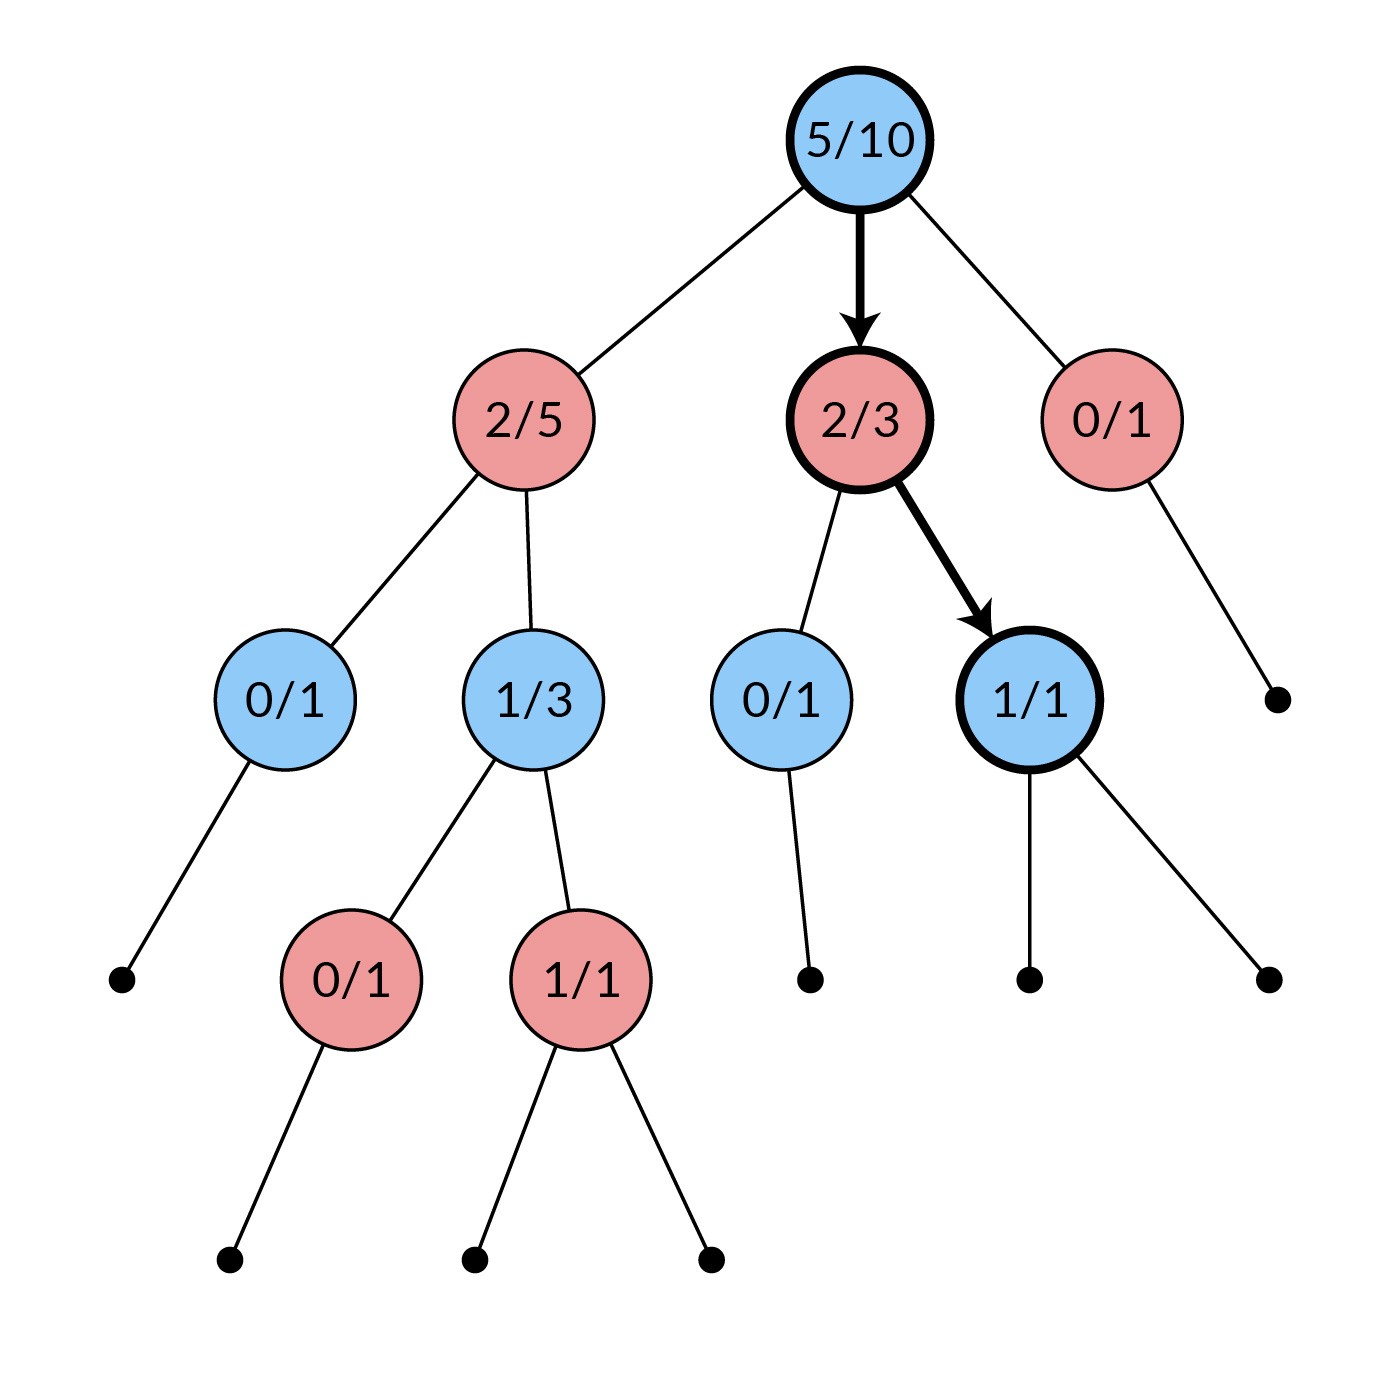
\includegraphics[width=0.6\textwidth]{figures/kap4/monte-carlo-tree-example.jpeg}
    \caption{Beispiel f�r einen Monte-Carlo-Suchbaum}
    \label{fig:monte-carlo-tree-example}
\end{figure}

Jeder Knoten hat einen Wert von \(Siege/Spiele\). Mit diesem Wert kann der beste Knoten basierend auf einem hohen Verh�ltnis von Gewinnen zu gespielten Spielen ausgew�hlt werden.